% Asset ID: AS1CoordinateGeometryCirclesTikZ-003
% Purpose: Show why side lengths are x-a and y-b.
\documentclass[tikz,border=8pt]{standalone}
\usetikzlibrary{calc,angles,quotes}
\begin{document}
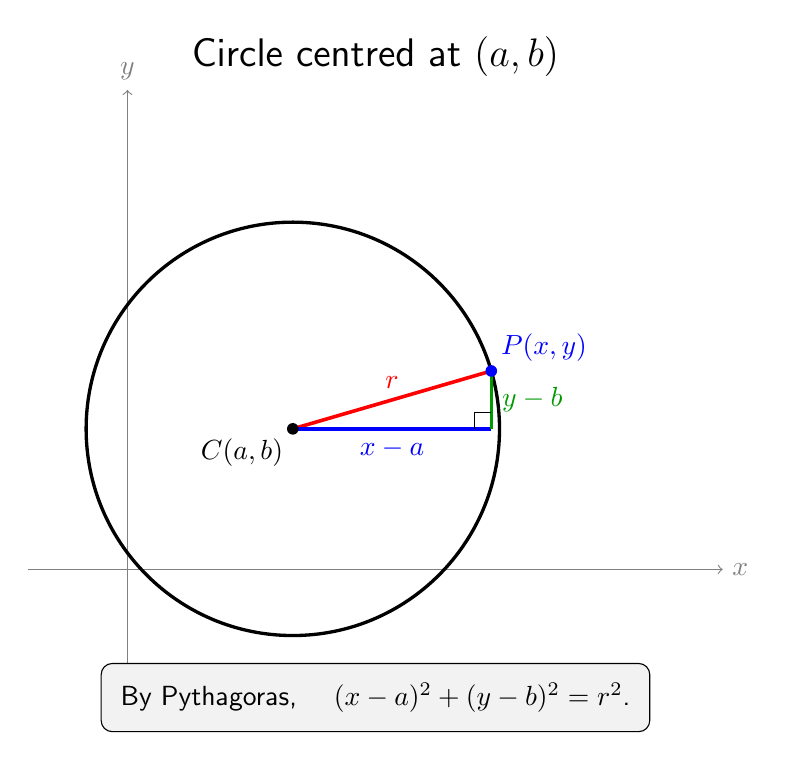
\begin{tikzpicture}[scale=1.05, font=\sffamily]
\draw[->, gray] (-1.2,0) -- (7.2,0) node[right] {$x$}; \draw[->, gray] (0,-1.2) -- (0,5.8) node[above] {$y$};
\coordinate (C) at (2,1.7); \draw[line width=1.2pt] (C) circle (2.5); \coordinate (P) at (4.4,2.4); \coordinate (Q) at (4.4,1.7);
\draw[line width=1.3pt, red] (C) -- (P) node[midway, above] {$r$}; \draw[line width=1.2pt, blue] (C) -- (Q) node[midway, below] {$x-a$}; \draw[line width=1.2pt, green!60!black] (Q) -- (P) node[midway, right] {$y-b$};
\fill[black] (C) circle (2pt) node[below left] {$C(a,b)$}; \fill[blue] (P) circle (2pt) node[above right] {$P(x,y)$}; \draw (4.2,1.7) -- (4.2,1.9) -- (4.4,1.9);
\node[align=center] at (3,6.2) {\Large Circle centred at $(a,b)$};
\node[align=center, draw, rounded corners, fill=gray!10, inner sep=7pt] at (3,-1.55) {By Pythagoras, \quad $(x-a)^2+(y-b)^2=r^2$.};
\end{tikzpicture}\end{document}
